\begin{figure}
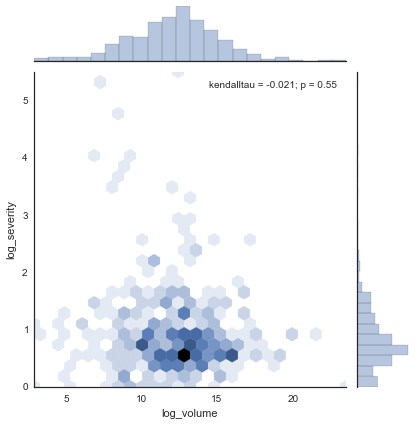
\includegraphics[width=\columnwidth]{severity_volume}
\end{figure}
\textcolor{red}{Is this section needed here? Looks like it is exactly as what's described in variables section.}

Our main outcome measures are the severity of the largest drop in the price of each asset (cryptocoin), and the magnitude (volume) of the transactions made with the cryptocoin measured in USD.
We scrape daily price and volume data from coinmarketcap.com \footnote{\textcolor{red}{For robustness analysis smaller subsets of the coins where available from coin}}.
%JULIAN: Didn't follow the above footnote
We operationalize the severity of a bubble as the inverse of 1 dollar that would be lost buying at the maximum price and selling after that proportionally to the volume of the market until the present; we call this severity.
%JUliAN: Above is hard to follow if not spelled out in the form of equations; wordy papers with everything explained inline seems more economics and less WWW
We define the volume as the sum of the dollar volume of trade reported over all exchanges.
